\lecture{11}{2026.05.25}{}

\subsection{Discrete Analog of Fourier Series}

Calculating the integration is very difficult in numerical coputing. Thus, we just consider some points on the function.

Given \[
    \{x_j, y_j\}_{j=0}^{2m-1}
\]
Consider $-\pi \le x \le \pi$ \[
    x_j = -\pi + \left(\frac{j}{m}\right)\pi, \quad j = 0, 1, \dots, 2m-1
\]
Assume $n < m$. Consider \[
    \{\phi_0, \dots, \phi_{2n-1}\}
\]
such that \begin{gather*}
\phi_0(x) = 
\frac{1}{2}\\
\phi_k(x) =
\cos kx, k = 1, \ldots, n\\  
\phi_{n+k}(x) =
\sin kx, k = 1, \ldots, n-1
\end{gather*}

\begin{definition}[Discrete Fourier Series]
    The apporximation function $S_n(x)$ \begin{align*}
        S_n(x) &= \frac{a_0}{2} + \sum_{k=1}^{n} a_k \cos kx + \sum_{k=1}^{n-1} b_k \sin kx \\
        &= \frac{a_0}{2} + a_n \cos nx + \sum_{k=1}^{n-1} (a_k \cos kx + b_k \sin kx) 
    \end{align*}
\end{definition}

The problem of least square approximation is to find $a_0, a_1, \dots, a_n$ and $b_1, \dots, b_{n-1}$ to minimize \[
    E = \sum_{j=0}^{2m-1} (y_j - S_n(x_j))^2
\]
That is \[
    \min_{a_0, a_1, \dots, a_n, b_1, \dots, b_{n-1}} \sum_{j=0}^{2m-1} \left(y_j - \frac{a_0}{2} - a_n \cos nx_j - \sum_{r=1}^{n-1} (a_r \cos rx_j + b_r \sin rx_j)\right)^2
\]

The situation becomes a multivariable optimization problem. First consider $1 \le k \le n$:
\begin{eqnarray*}
-\frac{\partial E}{\partial a_k} 
& = & \sum_{j=0}^{2m-1}
2 \biggl(y_j - (\frac{a_0}{2}
+ a_n \cos nx_j + 
\sum_{r=1}^{n-1} (a_r \cos rx_j 
+ b_r \sin r x_j)
)\biggr)\cos k x_j \\
& = & 
 2  \sum_{j=0}^{2m-1}
y_j \cos k x_j 
- 
2 a_k \sum_{j=0}^{2m-1}
\cos kx_j \cos k x_j - \red{2 \sum_{r=1, r \neq k}^{n} \sum_{j=0}^{2m-1}
a_r \cos rx_j 
\cos k x_j } - \\
&& \red{\sum_{j=0}^{2m-1}
a_0 \cos k x_j } - \red{2 \sum_{r=1}^{n-1} \sum_{j=0}^{2m-1}
b_r \sin r x_j \cos k x_j }
\end{eqnarray*}

If \begin{equation}
    \sum_{j=0}^{2m-1} \cos r x_j \cos k x_j = 0,\ k \neq r \label{eq:01}
\end{equation}
\begin{equation}
    \sum_{j=0}^{2m-1} \sin r x_j \sin k x_j = 0,\ 1 \le r \le n-1,\ 1 \le k \le n-1 \label{eq:02}
\end{equation}
and \begin{equation}
    \sum_{j=0}^{2m-1} \cos k x_j = 0, \label{eq:03}
\end{equation}
then we have \[
    \frac{\partial E}{\partial a_k} = 2 \sum_{j=0}^{2m-1} y_j \cos k x_j - 2 a_k \sum_{j=0}^{2m-1} \cos^2 kx_j = 0
\]

Similar to the continuous case, we hope \[
    \phi_0, \dots, \phi_{2n-1}
\]
are orthogonal with respect to the summation over equally spaced points $x_0, \dots, x_{2m-1}$ in $[-\pi, \pi]$.

\newpage

To prove \eqref{eq:01} to \eqref{eq:03}, we need the following theorem.

\begin{theorem}
    If $r$ isn't a multiple of  $2m$, then \[
        \sum_{j=0}^{2m-1} \cos r x_j = 0
    \mbox{ and }
        \sum_{j=0}^{2m-1} \sin r x_j = 0
    \]
\end{theorem}

Here is the proof of \eqref{eq:01}. From \[
    \cos r x_j \cos k x_j = \frac{1}{2} (\cos (r+k) x_j + \cos (r-k) x_j)
\]
Now \[
    1 \le r \le n,\ 1 \le k \le n,\ r \neq k
\]
then \[
    1 \le r+k \le 2n < 2m
\]
so $r+k$ isn't a multiple of $2m$. From the theorem, we have \[
    \sum_{j=0}^{2m-1} \cos (r+k) x_j = 0
\]
For $r-k$, we have \[
    -2m < -n \le r-k \neq 0 \le n < 2m
\]
so $r-k$ isn't a multiple of $2m$. Thus, \[
    \sum_{j=0}^{2m-1} \cos (r-k) x_j = 0
\]
Therefore, \[
    \sum_{j=0}^{2m-1} \cos r x_j \cos k x_j = 0
\]
The proof of \eqref{eq:02} is similar.

\vspace{1em}

Hence, we have \[
    \frac{\partial E}{a_k} = 2 \sum_{j=0}^{2m-1} y_j \cos k x_j - 2 a_k \sum_{j=0}^{2m-1} \cos^2 x_j = 0
\]
we must calculate \[
    \sum_{j=0}^{2m-1} \cos^2 k x_j
\]
which needs the following theorem.

\begin{theorem}\label{thm:1}
    If $r$ isn't a multiple of $m$, then \[
        \sum_{j=0}^{2m-1} \cos^2 r x_j = m
        \mbox{ and }
        \sum_{j=0}^{2m-1} \sin^2 r x_j = m
    \]
\end{theorem}

\vspace{0.5em}

If \[
    1 \le k \le n < m
\]
we have $k$ isn't a multiple of $m$. By the theorem, \[
    \sum_{j=0}^{2m-1} \cos^2 k x_j = m
\]

Finally, we have \[
    a_k = \frac{1}{m} \sum_{j=0}^{2m-1} y_j \cos k x_j, \quad k = 1, \dots, n
\]
We now need to handle the case $k = 0$. We have 
\begin{eqnarray}
- \frac{\partial E}{\partial a_0}  &= & 
 2  \sum_{j=0}^{2m-1}
\left(y_j 
- 
\frac{a_0}{2}
- \sum_{r=1}^{n} a_r \cos rx_j - \sum_{r=1}^{n-1}
   b_r \sin rx_j \right) \frac{1}{2} \nonumber \\
&=&
2 \sum_{j=0}^{2m-1} \left(y_j - \frac{a_0}{2}\right) \frac{1}{2} 
- \sum_{r=1}^{n}
a_r \sum_{j=0}^{2m-1} \cos rx_j - \sum_{r=1}^{n-1} b_r \sum_{j=0}^{2m-1} \sin r x_j  \label{eq:1} \\
&= &2 \sum_{j=0}^{2m-1} \left(y_j - \frac{a_0}{2}\right) \frac{1}{2} = 0 \nonumber
\end{eqnarray}

Note that in \eqref{eq:1}, we use the result from a Theorem~\ref{thm:1}. Now we have \[
    \sum_{j=0}^{2m-1} y_j - m a_0 = 0
\]
Since \[
    \cos kx_j = 1 \mbox{ if } k=0,
\]
we can write $a_0$ as \[
    a_k = \frac{1}{m} \sum_{j=0}^{2m-1} y_j \cos k x_j, \quad k = 0
\]
This has the same form as the case $k = 1, \dots, n$. 

\begin{note}
    Which explain that why we need to define $\frac{a_0}{2}$ instead of $a_0$.
\end{note}

Similarly, we get \[
    b_k = \frac{1}{m} \sum_{j=0}^{2m-1} y_j \sin k x_j, \quad k = 1, \dots, n-1
\]

\begin{remark}
The derivation require $n < m$, which means when $k = n = m$, \[
    \frac{\partial E}{\partial a_m} = 2 \sum_{j=0}^{2m-1} y_j \cos m x_j - 2 a_m \sum_{j=0}^{2m-1} \cos^2 m x_j = 0
\]
Note that \[
    x_j = -\pi + \left(\frac{j}{m}\right) \pi, \quad j = 0, 1, \dots, 2m-1
\]
Thus, we have \[
    \cos^2 m x_j = \cos^2 (j-m) \pi = 1
\]

Then \[
    a_m = \frac{1}{2m} \sum_{j=0}^{2m-1} y_j \cos m x_j,
\]
is different from the general form. It has $\frac{1}{2m}$ instead of $\frac{1}{m}$. 

\vspace{1em}

To get the same form \[
    S_n(x) = \frac{a_0 + a_n \cos nx}{2} + \sum_{k=1}^{n-1} a_k \cos kx + \sum_{k=1}^{n-1} b_k \sin kx
\]

Therefore $n = m$ is also fine though earlier we used
$n < m$ in our derivation.
\end{remark}

\begin{note}
    In the later discussion of the Fast Fourier Transform, we will see that the case $n = m$ is more important than the case $n < m$.
\end{note}

\begin{eg}
    Let \[
        f(x) = x^4 - 3x^3 + 2x^2 - \tan (x(x-2))
    \]
    Given $m=5 \implies 10$ points \[
        (x_j, y_j),\ j = 0, 1, \dots, 9 \quad \quad x_j = \frac{j}{5},\ y_j = f(x_j)
    \]
\end{eg}

\vspace{0.5em}

Need to \red{linearly transform} these points to $[-\pi, \pi]$ \[
    z_j = \pi (x_j - 1)
\]
Data become \[
    z_j,\ f\left(1 + \frac{z_j}{\pi}\right),\ j = 0, 1, \dots, 9
\]
Let $n = 3$, least square trigonometric approximation is \[
    S_3(x) = \frac{a_0}{2} + a_3 \cos 3z + \sum_{k=1}^{2} (a_k \cos kz + b_k \sin kz)
\]
where \[
    a_k = \frac{1}{5} \sum_{j=0}^{9} f\left(1 + \frac{z_j}{\pi}\right) \cos kz_j, \quad k = 0, 1, 2, 3
\]
and \[
    b_k = \frac{1}{5} \sum_{j=0}^{9} f\left(1 + \frac{z_j}{\pi}\right) \sin kz_j, \quad k = 1, 2
\]

Here is the MATLAB code to calculate the coefficients 
\begin{minted}[linenos, bgcolor=LightGray]{matlab}
m = 5;
x=[0:1:2*m-1]' / 5;
y = x.^4 - 3 * x.^3 + 2 * x.^2  - tan(x .* (x-2));
z = pi * (x-1);
n = 3;
a = []; b = [];
for k=0:n
    a = [a ; 1/m * sum(y .* cos(k * z))];
end
for k=1:n-1
    b = [b; 1/m * sum(y .* sin(k * z))];
end
approx = a(1)/2 + cos(z*(1:n))*a(2:n+1) + sin(z*(1:n-1)) * b(1:n-1)
\end{minted}

\begin{minted}[frame=single,framerule=1pt,  rulecolor=\color{gray}]{matlab}
>> [y approx]
ans =
         0    0.0011
    0.4340    0.4178
    0.8981    0.9107
    1.3172    1.3208
    1.5820    1.5716
    1.5574    1.5578
    1.1980    1.2079
    0.6452    0.6414
    0.1301    0.1188
   -0.1420   -0.1278
\end{minted}

\begin{figure}[H]
    \centering
    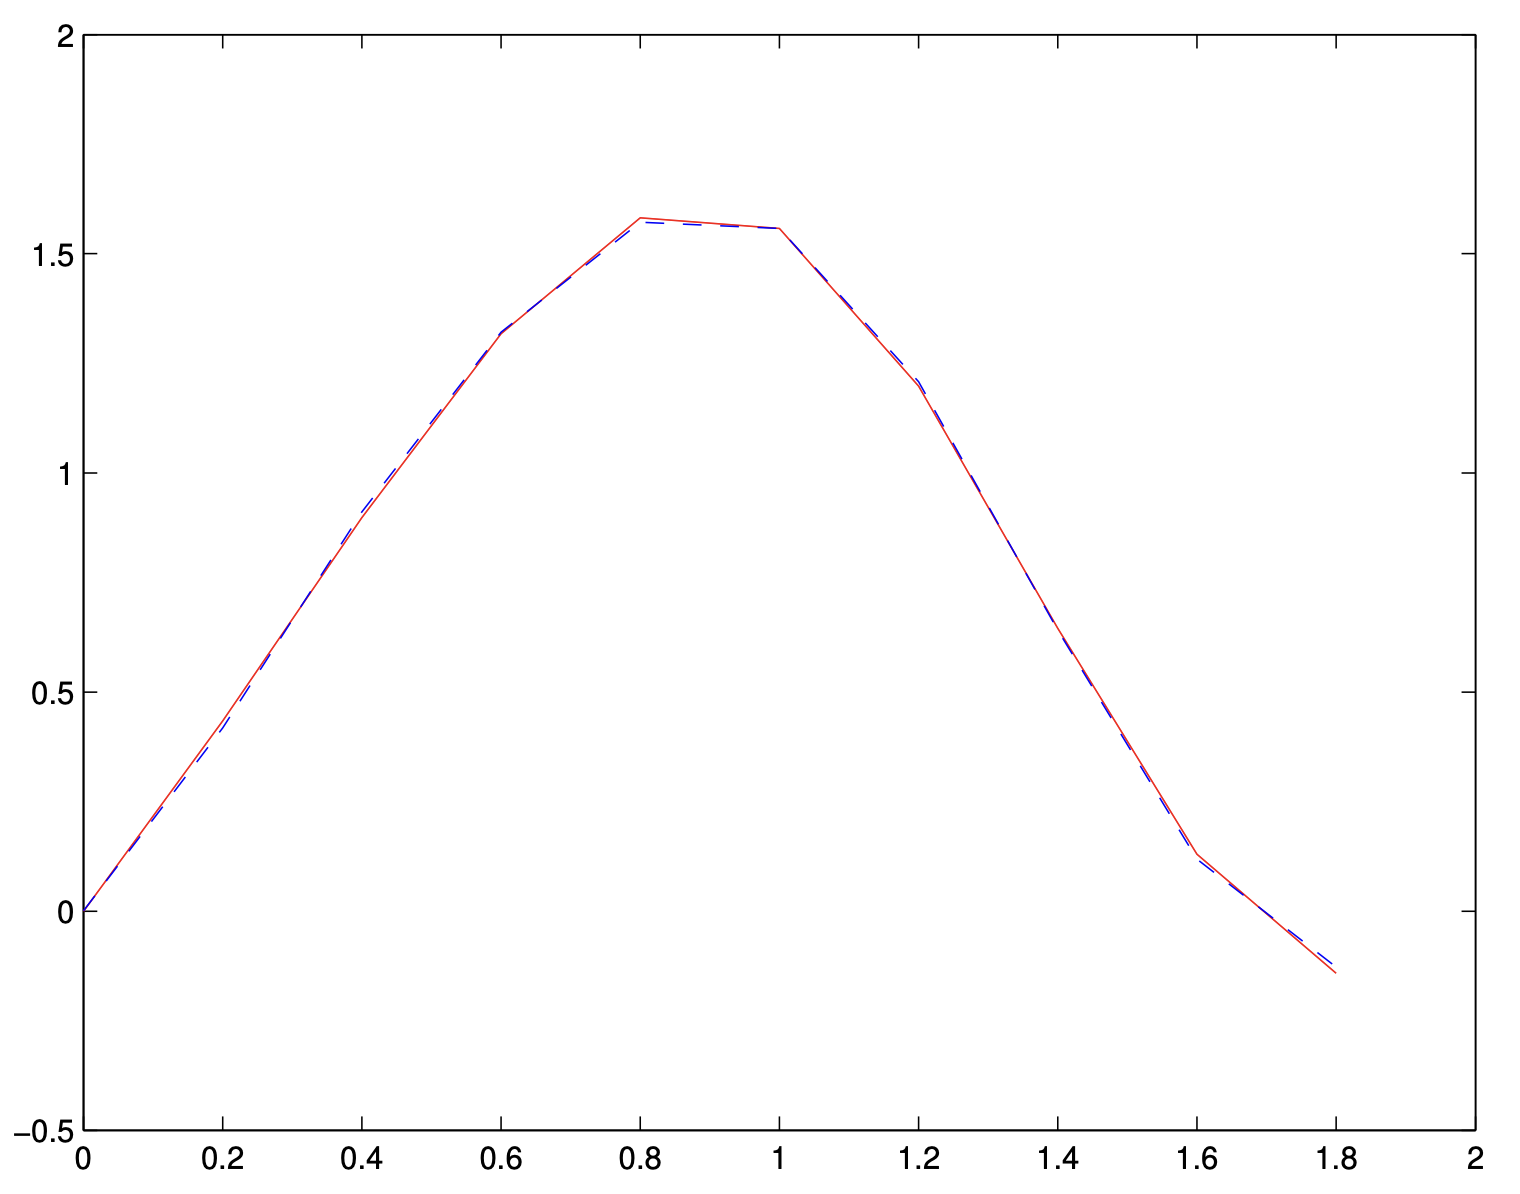
\includegraphics[width=0.6\textwidth]{Figures/FTex.png}
    \caption{Fourier approximation of $f(x)$}
\end{figure}